\documentclass[12pt,a4paper]{article}
\usepackage{enumerate} %put in numbers or bullet points
\usepackage{setspace}
\raggedright %justify the text on the left only
\usepackage{graphicx} 	% For adding pictures
\usepackage{float}
\usepackage{pdflscape}	% for landscape pages
\pagenumbering{arabic}	% Page numbers
\usepackage{fancyhdr} % add headers and footers
\usepackage{hyperref} % hyper links for references

\onehalfspacing %1.5 line spacing
\usepackage[round]{natbib} % author-year citations in round brackets


\begin{document}

\title{Morphological disparity in the evolution of tenrecs}
\author{}
\date{}
\maketitle


%Add a header 
\renewcommand{\headrulewidth}{0.0pt}
\thispagestyle{fancy}				%header on the first page only
\lhead{Sive Finlay, Progress Report}
\chead{}
\rhead{September 2014}


\section{Overview}
My research is an investigation of evolutionary patterns in tenrecs (Afrosoricida,  Tenrecidae). The original aim of my project was to quantify both morphological and ecological diversity within the tenrecs family (disparity) and their similarities to other small insectivorous mammals (convergence). I have almost completed the first part of this plan; please see the paper draft "Cranial morphological disparity within the adaptive radiation of tenrecs (Afrosoricida, Tenrecidae) is no greater than expected by chance" which accompanies this report.

After much careful consideration and seeking advice from many different sources, I have decided to convert my project to a Masters by research thesis rather than PhD. My plan is to use the attached paper as the basis for the thesis along with a more extensive introduction and conclusion as well as a more detailed methods section. 

I have not made this decision lightly but I believe that it is the best option for me. If I were to continue with my project then officially I would have one year left to complete the PhD. However, realistically I know that it would take much longer. My plan was to have seven chapters: four of which would be paper driven along with an introduction, data collection and conclusions. The accompanying paper would be one of the four paper-driven chapters. The others would be 1) a review of methods of quantifying convergence, 2) quantifying morphological convergence among tenrecs and other small mammals, 3) testing whether morphological convergence is predicted by ecological similarity. In my first year report in November 2013 (see attached document) I included an outline for a further chapter based on behavioural studies of echolocatory capabilities in shrew-type (\textit{Microgale}) tenrecs. Natalie and I travelled to Madagascar in April of this year but unfortunately our experiments were unsuccessful so I was unable to collect sufficient data for this chapter.

Completing this PhD thesis plan would be more than a simple extension of the work that I'm doing already. I would need to master different statistical techniques for quantifying convergence to a sufficient degree to be able to both use the methods for my own research and to critique them in a review. Furthermore, I would need to collect a new data set of ecological variables for my species and then apply different methods for assessing the evidence for ecological convergences among tenrecs.
I understand that it's common to feel overwhelmed by a PhD half way through the project. However, my decision to switch to a masters instead is not purely a matter of being overwhelmed or unwilling to approach hard work. Despite the volume of work remaining I know that I do have the ability to complete the project if necessary. However, my strengths and interests lie outside traditional research and I don't wish to continue struggling to finish a piece of work to which I'm not suited.

I am extremely grateful to the committee for all of your help and guidance over the past two years. I feel especially thankful and fortunate to have had such a dedicated supervisor: I am so grateful to Natalie for her constant support, mentoring, teaching and advice.   

In this report I outline the current progress on my paper, plans for how I will develop the work into a complete Master's thesis and a brief summary of the other academic work completed since my last report. I would be very grateful for advice about what's the best way to approach this transition. My current plan is to contact the IRC this month (September) to tell them that I would like to terminate my contract and that they should close my research account with college.
 
My fees are covered by my final year of Schols so I would like to re-register as a student for this academic year. My aim is to complete and hopefully submit the paper by mid-October and then work it up into at least a first draft of a full thesis by mid November to be ready to submit before the end of the semester. However, if I submit the thesis before Christmas would that make me inelligible to re-register as a continuing student in January? If so then I would prefer to wait and submit my thesis after re-registering. These options are pretty much equivalent in the long term because, all going well, my year of graduation from the masters would be 2015 either way. Therefore I would be grateful for advice on what's the best way to ensure that I'm elligible to remain a student for the full 2014/2015 academic year.


\section{Progress on the accompanying paper}

Chapter 3: Quantifying morphological disparity in tenrecs
\textit{Journal targets: Journal of Evolutionary Biology, PLoS ONE, Journal of Mammalian Evolution? , submit August 2014.} 


This is the chapter which corresponds to the draft paper that accompanies this report. I have completed the majority of the work for this paper. Given that tenrecs are often cited as an example of a phenotypically diverse group \citep[e.g.][]{Olson2013}, my finding that morphological disparity is no greater than expected by chance was unexpected. Therefore I'm currently checking the code that I used for the calculations and simulation studies to ensure that the results are accurate rather than just artefacts of a fault in the methods. 

I would very much welcome any comments on the draft paper, particularly if you have suggestions for how I could make the overall story clearer and more interesting to a wide audience. My aim for the paper is that it's a test of a broad principle; the importance of testing our assumptions about phenotypic variation in adaptively radiated groups, with tenrecs as a specific example rather than a more limited study of morphological variation in a particular group of mammals.

Dr. Steve Goodman, an expert in tenrec ecology and evolution, has expressed an interest in collaborating on the paper so I will send it to him for comments before submitting to the Journal of Evolutionary Biology by the end of the summer.


\section{Extending the paper into a thesis}


%Re-write this section about introduction, data collection and conclusion

This is a general introductory chapter. I will include brief outlines of convergence and disparity and why they are useful and interesting measures of evolutionary diversity. I will discuss convergence within the context of what it tells us about the repeatability of evolution \citep[e.g][]{Blount2008} and disparity within the framework of how it relates to the study of adaptive radiations \citep{Losos2010a}. In particular, I will stress the importance of taking quantiative approaches to studying each of these patterns rather than relying on subjective estimates. I will follow these discussions with a brief introduction of tenrecs and the long-standing interest in the apparently high morphological and ecological diversity within the family and the similarities among tenrecs and other distantly related mammal species \citep[e.g.][]{Eisenberg1969, Soarimalala2011, Olson2013}. 

Along with the conclusions (chapter seven), this will be the last chapter that I write because it will be easier to introduce the rest of the thesis once I know how those chapters have taken shape. 

\textbf{Chapter 2: Data collection}\\

My thesis will be based on two main data sources; morphological and ecological. The questions addressed in chapters three, five and six will all be base on these same data sources. Therefore, rather than repeating the information in multiple sections, I will combine my data collection methods into this single chapter which I can then refer to in the rest of the thesis. 
I have collected all of the data and completed most of the writing for the morphological section of this chapter. I haven't started the sections relating to the ecological data but I will work on this aspect as I collect the relevant data over the coming months (see chapter six below). I will finish writing the chapter by this September.



\textbf{Chapter 7: Conclusions}\\


This chapter will summarise the importance of taking a quantitative approach to studies of evolutionary diversity (morphological and ecological) among species groups. In particular I will highlight the need to apply existing methods to new groups of species which are usually not as well studied as the groups that are used to develop such metrics. I will also include suggestions for future directions, particularly in the area of addressing the functional importance rather than pure description of convergent traits \citep{Losos2010}. I could also include mention my unsuccessful fieldwork experiments here (see below) as another potential basis for future work. 



%I don't think this is relevant any more
%\section{Unsuccessful fieldwork for testing behavioural convergence}

%In my November 2013 report I outlined my plans for incorporating tests of behavioural convergence into my project. I was interested in whether early reports of an ability to echolocate in some tenrecs \citep{Gould1965} may be extended to other species of the \textit{Microgale} (shrew-type) tenrecs and therefore provide evidence of behavioural convergence between tenrecs and shrews \citep{Siemers2009}. Natalie and I went to Madagascar in March/April as part of a research trip led by Dr.Steve Goodman to conduct behavioural tests of echolocation in \textit{Microgale}. Our aim was to record the sounds made by the animals as they moved through a wooden maze towards a food reward to determine whether there was evidence that they were using sounds to navigate through their environment. We tried multiple variations of our protocol but unfortunately none of the animals we tested produced any noise (17 individuals from 5 different species). It is clear that this negative result is a failure of our experiment rather than an indication that \textit{Microgale} don't navigate using sounds. Our sample included \textit{Microgale dobsoni} which are one of the few species which are known to echolocate from previous experiments \citep{Gould1965}. Similarly, other more experienced researchers in the group had heard the \textit{Microgale} making sounds while foraging. Previous studies of echolocation in small mammals \citep{Gould1964, Gould1965, Tomasi1979, Siemers2009} all used captive individuals which were trained to perform specific tasks. Such a prolonged procedure was not possible wihtin our constraints of time and facilities.

%Given that I have no useable data to address my questions of behavioural convergence it is not enough information for a complete chapter. I could mention the experiments briefly in my concluding chapter as an idea for further directions. Alternatively, I could leave these investigations of behavioural convergence out of the thesis altogether to avoid detracting from my more general studies of morphological and ecological (dis)similarities among species.

%Could probably take this out too
\section{Other work}
\begin{enumerate}

\item \textbf{Publications since the November 2013 report}\\
\textbf{Finlay, S.}, Goodman, S.M., Cooper, N. Significant levels of morphological disparity in the adaptive radiation of tenrecs (Afrosoricida, Tenrecidae). \textit{In prep. To be submitted to the Journal of Evolutionary Biology}\\
\bigskip %skip a line between the two references
Healy, K., Guillerme T., \textbf{Finlay, S.,}, Kane, A., Kelly, S.B.A., McClean, D., Kelly, D.J., Donohue, I., Jackson, A.L. and Cooper, N., 2014.Ecology and mode-of-life explain lifespan variation in birds and mammals. \textit{Proceedings of the Royal Society B, 281(1784)} 

\item \textbf{Presentations}\\
This summer I gave my first oral conference presenations at the Evolution conference in Raleigh, North Carolina (June) and the British Ecological Society Macroecology conference in Nottingham (July).

\item \textbf{Reviewing}\\

So far I have reviewed a journal article (International Journal of Primatology) and a book chapter on phylogenetic comparative methods for quantifying convergence. I hope that I will get some more reviewing practice once I start publishing my own papers.



\end{enumerate}

%Do I need a GANNT chart?

%\begin{landscape}
%\begin{figure}[p]
%\centering
%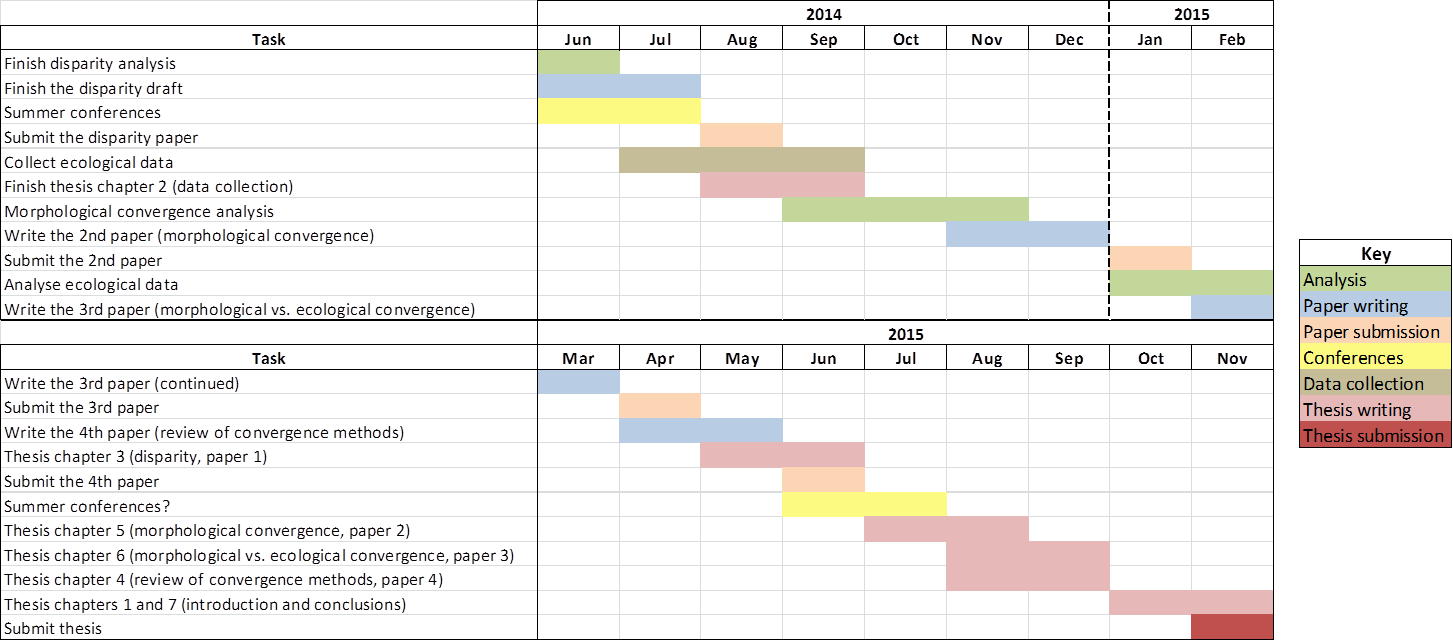
\includegraphics[keepaspectratio=true]{Gannt+key.png}
%\caption{Timeline for completion of my PhD, tasks are colour coded following the accompanying key}
%\label{gannt}
%\end{figure}
%\end{landscape}



\bibliographystyle{jeb}
\bibliography{Refs_01_05_14_edited} %This is my edited JabRef file of all my references exported from EndNote. I had to edit the formatting for the special characters, capital letters and also change the file encoding.


\end{document}